\section{Topic Modeling Evaluation}

    \graphicspath{{Chapter4/Figures}{Chapter4/Figures}}

In this chapter, the evaluation of different models used for tweet labeling is presented. Both unsupervised and supervised approaches were used to evaluate the performance of the models. 
The goal of the evaluation was to find the best-performing model to accurately label tweets. 
The models used included traditional methods (LDA, GSDMM, and NMF) as well as neural models like  BERTopic. Evaluation metrics such as coherence and diversity were used to compare the different models. The results showed that BERTopic performed better than traditional methods, especially when using all-MiniLM-L6-v2 (BERT) \footnote{\href{https://huggingface.co/sentence-transformers/all-MiniLM-L6-v2}{huggingface.co/sentence-transformers/all-MiniLM-L6-v2}}
, text-embedding-ada-002 (OpenAI) \footnote{\href{https://platform.openai.com/docs/models/embeddings}{platform.openai.com/docs/models/embeddings}}, and tweet\_classification \footnote{\href{https://huggingface.co/louisbetsch/tweetclassification-bf-model}{huggingface.co/louisbetsch/tweetclassification-bf-model}} embeddings. The supervised evaluation showed that BERT and OpenAI were the best-performing models. The section concludes with a summary of the results and a description of the representation used for labeling the tweets.

The models used are both traditional(LDA, GSDMM, NMF) as a reference of the ground truth and neural because seem to be the most accurate, in particular, we will evaluate BERTopic with several embedding methods. We choose BERtopic over Top2Vec because they are very similar and also because the Python library is more complete and allows us to be more flexible.

Evaluating a topic modeling algorithm is not a straightforward task due to the lack of objectivity in identifying a topic. In this work we evaluated the models in two ways: first using a widely used unsupervised approach: metrics like coherence and diversity. 
Then to validate the results we also did a supervised evaluation using different datasets built ad hoc for this setting.

\subsection{Unsupervised}
To compare the different models we used a library suggested by the creator of BERtopic called OCTIS \cite{DBLP:conf/clic-it/TerragniF21} \cite{terragni2020octis}, this allowed us to structure an experiment to measure different metrics:

\paragraph{Metrics}

\begin{itemize}
    \item \textbf{NPMI coherence:} degree of association between the top words in a topic
    \item \textbf{Umass coherence}: how often two words appear together
    \item \textbf{Diversity}: how distinct the topics are from each other
    \item \textbf{Computation time}: time needed to fit the models
\end{itemize}


\paragraph{Dataset}
In this case, the dataset is composed of 1669 preprocessed tweets related to climate change with the hashtag \textit{\#cop22}, the preprocessing phase involved removing retweets, links, punctuation, and the most common hashtags (\#cop22, \#climatechange \#p2), all the tweets were in English.

\paragraph{Methods}

The models used in this evaluation were: LDA, NMF, and BERTopic. In the BERtopic case, several embeddings have been tested (  all-MiniLM-L6-v2, text-embedding-ada-002, climatebert \cite{webersinke_climatebert_2022}, tweet\_classification, USE \cite{cer_use_2018}).

Each model has been fitted several times changing the parameters:
\begin{itemize}
    \item  \textbf{number of topics} from 10 to 50 with a step of 5 
    \item \textbf{min topic siz}e: 5 and 15 \footnote{only for bertopic}
\end{itemize}


Each unique combination of parameters has been fit 3 different times, then we took the mean value of the 3 computations.

\paragraph{Results}
The results show that BERtopic performs way better in these tests than the traditional methods. While the best Bertopic embeddings are mini, OpenAi, and tweet classification.

The experiment demonstrates how the \textit{min\_topic\_size} value of 5 is too small, so the results will be with a value of 15.

Fig \ref{figure:unsupervised_results} shows the value of all the metrics with a different number of topics for the traditional methods and the best-performing neural one (OpenAI)

\begin{figure}[h]
    \centering % figure is centered on the page
        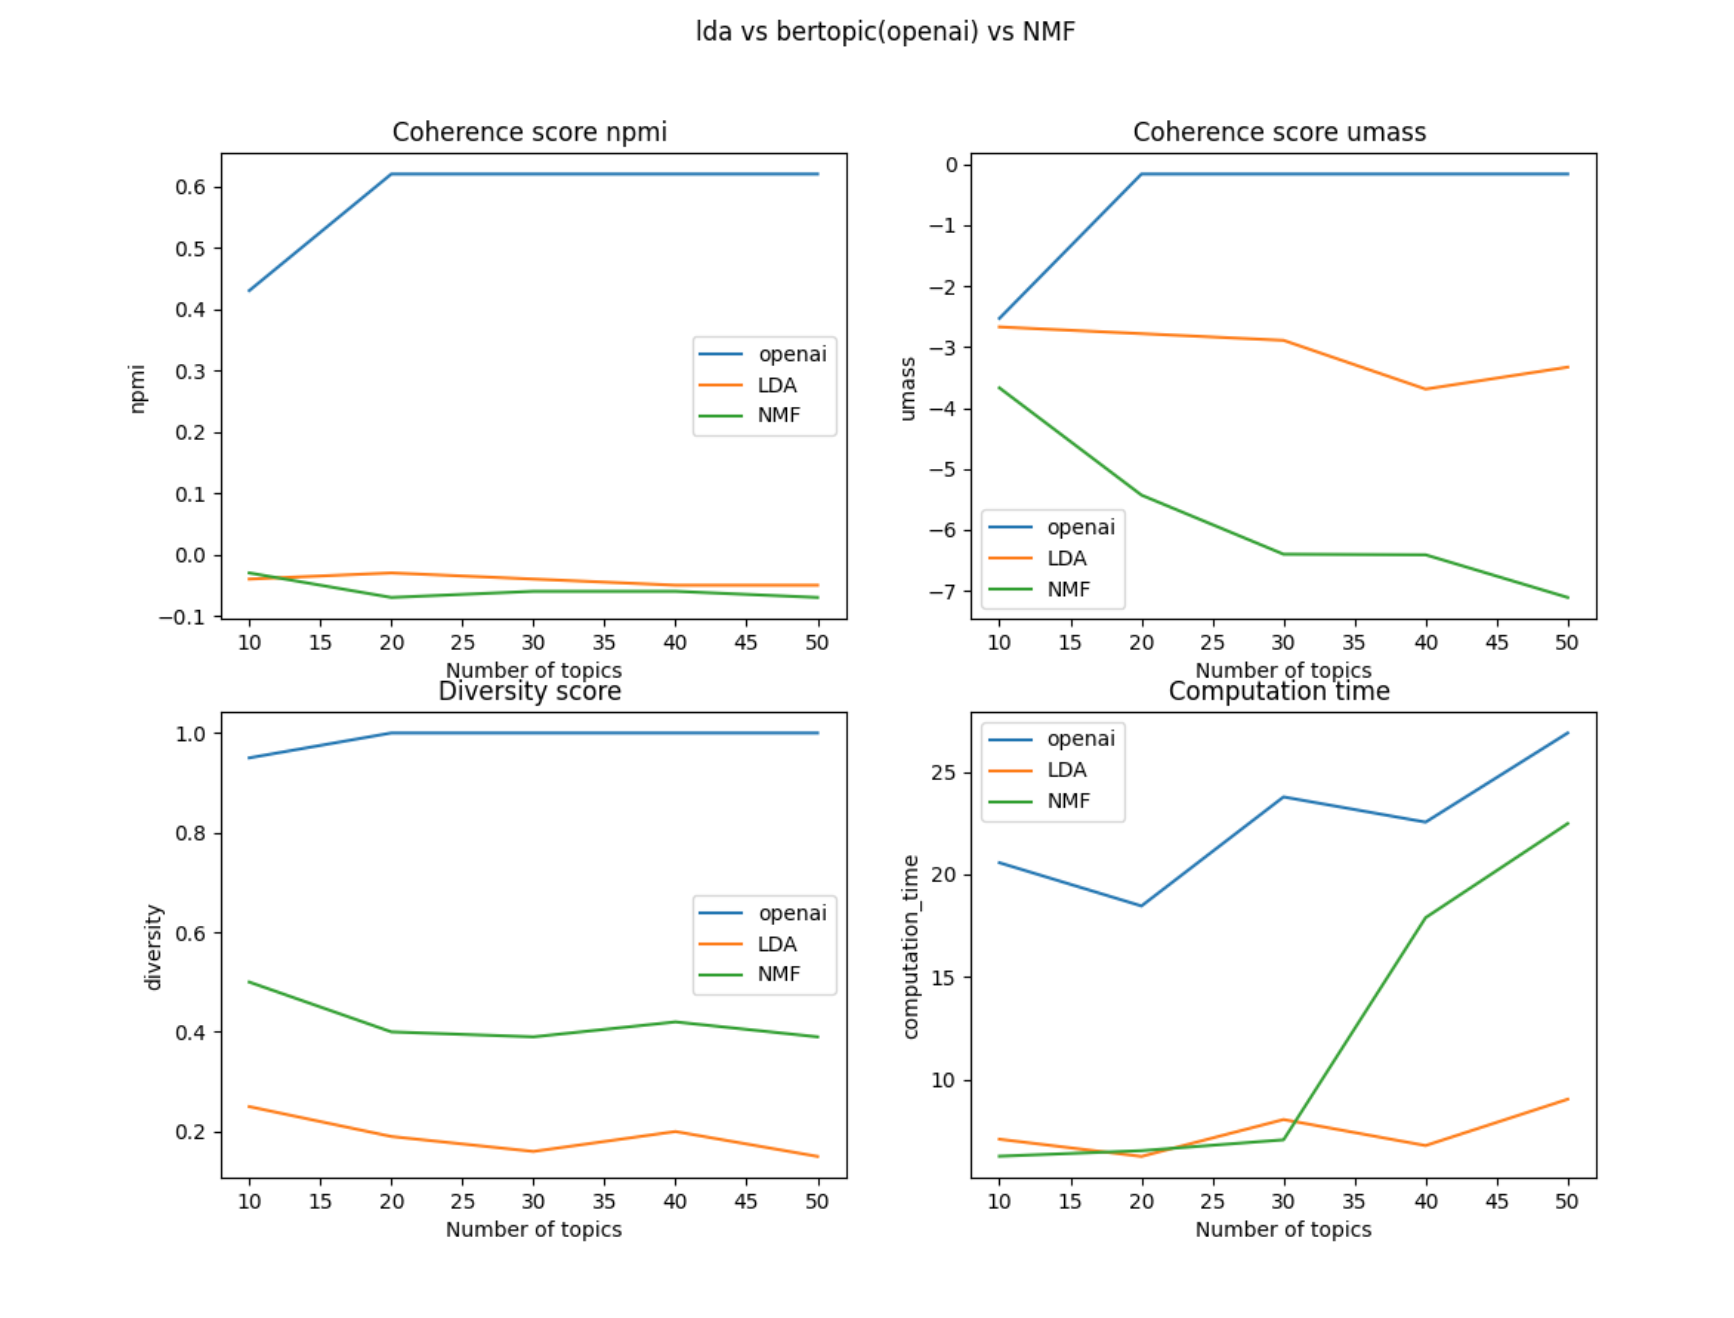
\includegraphics[width=0.99\linewidth]{Chapter4/figures/topic_unsupervised.png} 
    \caption{coherence and diversity for LDA, BERTopic, and NMF
    }
    \label{figure:unsupervised_results} % assign a unique label to each figure
\end{figure}


However, Hoyle et al  \cite{hoyle_is_2021} showed how these metrics are not very meaningful for evaluating these models and we should take these results with a grain of salt.

From this evaluation, we can conclude that for BERTopic the topic size is better bigger than smaller especially if we have many documents. Topics of Bertopic are way more diverse than LDA and NMF and within the topics, the most relevant word are more semantically related.


\subsection{Supervised}
Considering the result of the unsupervised evaluation we should use another method to validate what we found. In this case, we created two ad hoc datasets to see too how the models perform in a real-case scenario.

\paragraph{Dataset}

The first step for the supervised part was the data collection, in this case, we packed specific datasets to test our models. The first is simpler and contains very different topics so that should be easy to cluster the documents, while the second is more trickier because it contains only politics-related tweets with some overlapping.

\begin{itemize}
    \item \textbf{simple}: 1093 labeled tweets of 5 different topics identified by a hashtag \footnote{\#Bitcoin, \#stormydaniels, \#UkraineRussianWar, \#SaudiArabianGP, \#climatechange}
    \item \textbf{politics}: 1492 labeled tweets of 7 politics-related hashtags \footnote{\#IndictArrestAndConvictTrump, \#kabul, \#BidenHarris2024, \#KamalaHarris, \#taiwan, \#belarus,  \# stormydaniels}
\end{itemize}


For both datasets, we used two different versions: with and without hashtags.

The tweets have been extracted using \href{https://twarc-project.readthedocs.io/en/latest/twarc2_en_us/}{twarc2} getting only English tweets and without retweets.

\paragraph{Metrics}
In order to evaluate the topics we had to define some metrics:

\begin{itemize}
    \item \textbf{Accuracy}: for each known topic look at the biggest of inferred topics and divide by the number of tweets in that topic.
    \item \textbf{Accuracy no outliers}: in the Bertopic case the label -1 refers to outliers.
    \item \textbf{Min\_topic\_share}:  same as accuracy but in the opposite direction, after having computed it for all of my\_topics we take the minimum
\end{itemize}


\paragraph{Parameters}

\begin{verbatim}
BERTopic: (nr_topics = 'auto', min_topic_size = 50)

NMF: (max_df = 0.95, min_df = 3, ngram_range = (1,2))

GSDMM: (alpha = 0.1, min_df = 0.1, n_iters = 30)
\end{verbatim}


\paragraph{Simple Dataset Results}
We started evaluating the \textit{simple} dataset with hashtags and as we can see in Fig \ref{figure:supervised bar} base ( all-MiniLM-L6-v2) and OpenAi obtained almost a perfect score for each topic, while climatebert seems to have a great accuracy but a low mean topic share, this is a signal that something is wrong and we should inspect the heatmap.

\begin{figure}[h]
    \centering % figure is centered on the page
        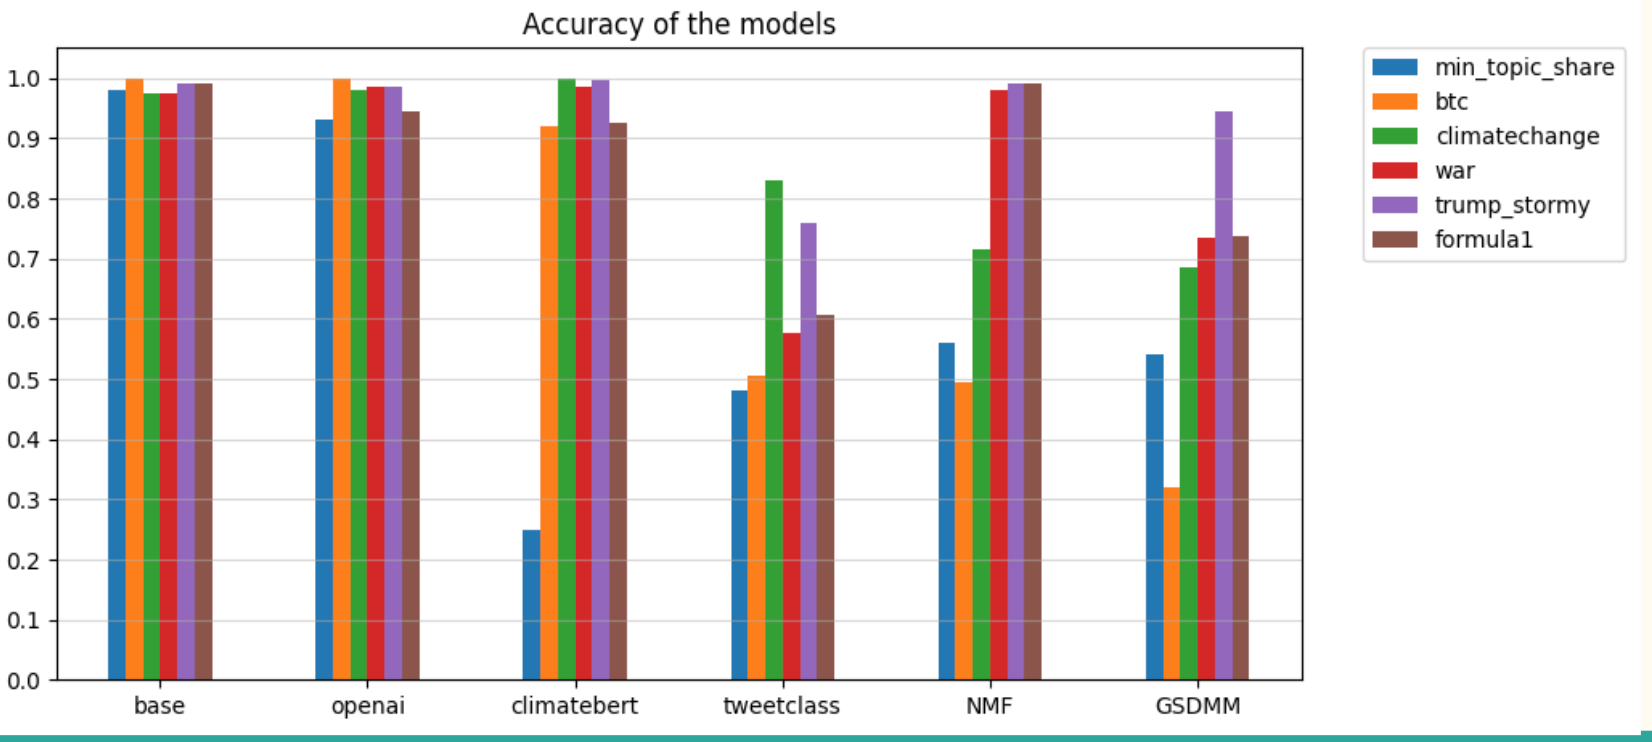
\includegraphics[width=0.99\linewidth]{Chapter4/figures/topic_supervised_bar.png} 
    \caption{All models accuracy simple  with hashtags
    }
    \label{figure:supervised bar} % assign a unique label to each figure
\end{figure}

In fact, we can clearly see in \ref{figure:sup_heatmap1_simple_hash} that even though the accuracy is very good, climatebert has some difficulties in dividing the topics putting almost all the tweets in the same. While the first two are performing very well as expected it is not true for the others. We can see how climate bert put almost all the tweets in topic 0, being able only to find the formula1 tweets and not the climatechange one, as it is designed to do.
That’s the reason why we decided to remove the models that are not performing well in the simplest case with the exception of NMF to use it as ground truth. 


\begin{figure}[h]
    \centering % figure is centered on the page
        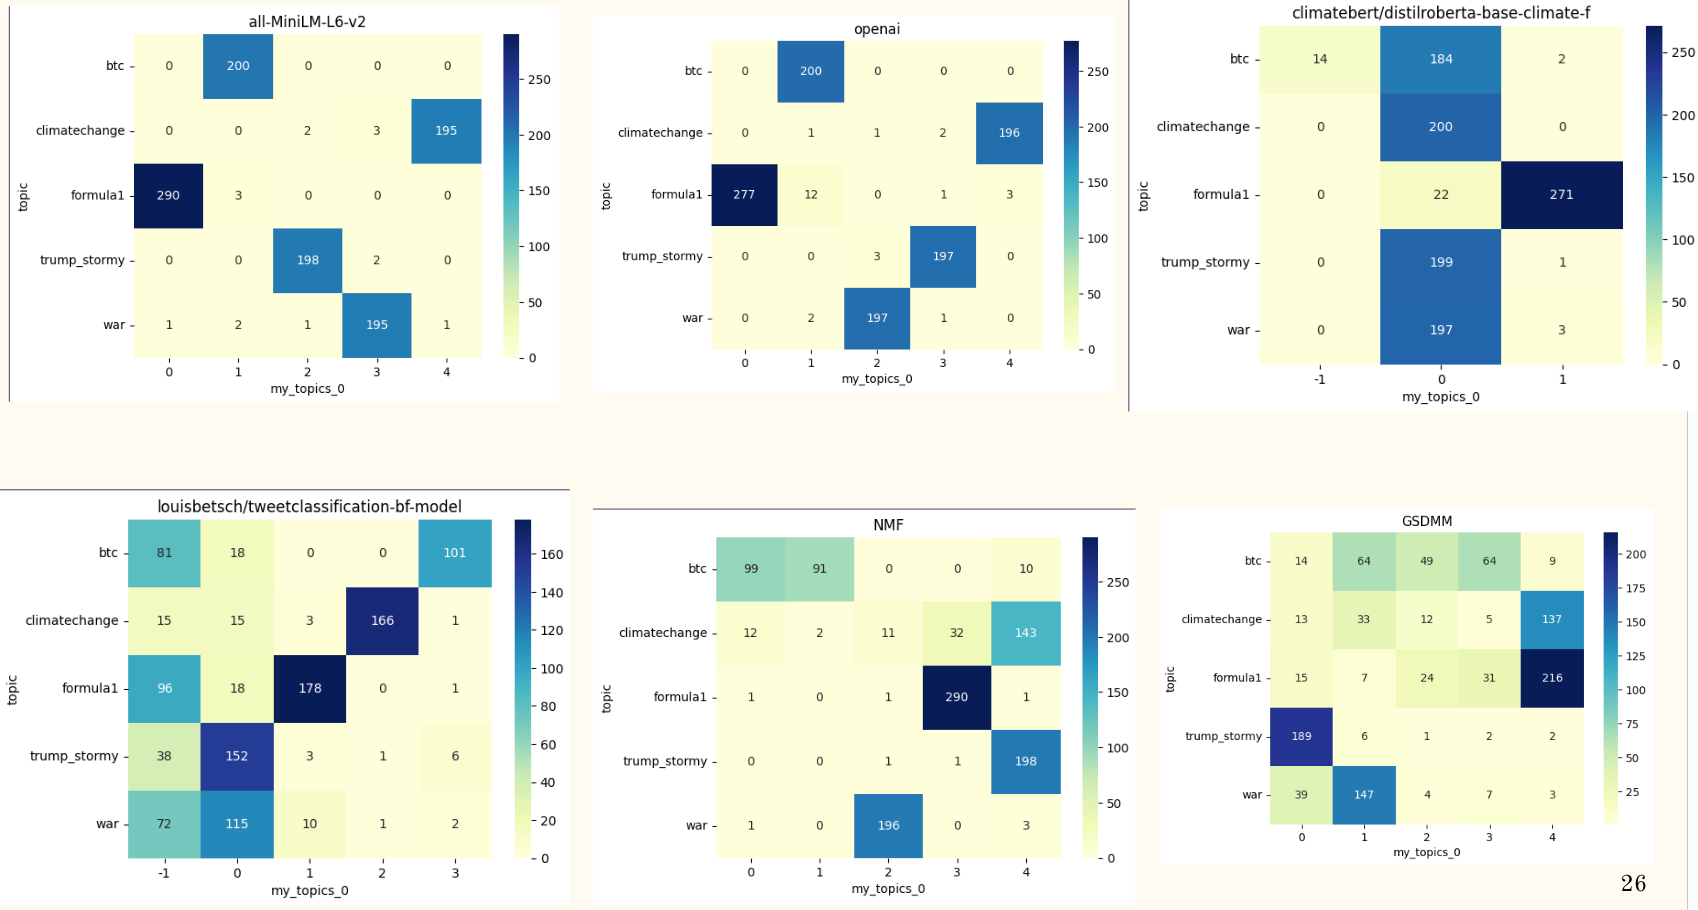
\includegraphics[width=0.99\linewidth]{Chapter4/figures/topic_heatmap1.png} 
    \caption{Heatmap comparison of the different model with the simple dataset with hashtags
    }
    \label{figure:sup_heatmap1_simple_hash} % assign a unique label to each figure
\end{figure}

Looking at \ref{figure:supervised heatmap1} we can see how BERT and OpenAI performed in the same dataset but without the hashtags, in particular how BERT tends to find more outliers than OpenAI.


\begin{figure}[h]
    \centering % figure is centered on the page
        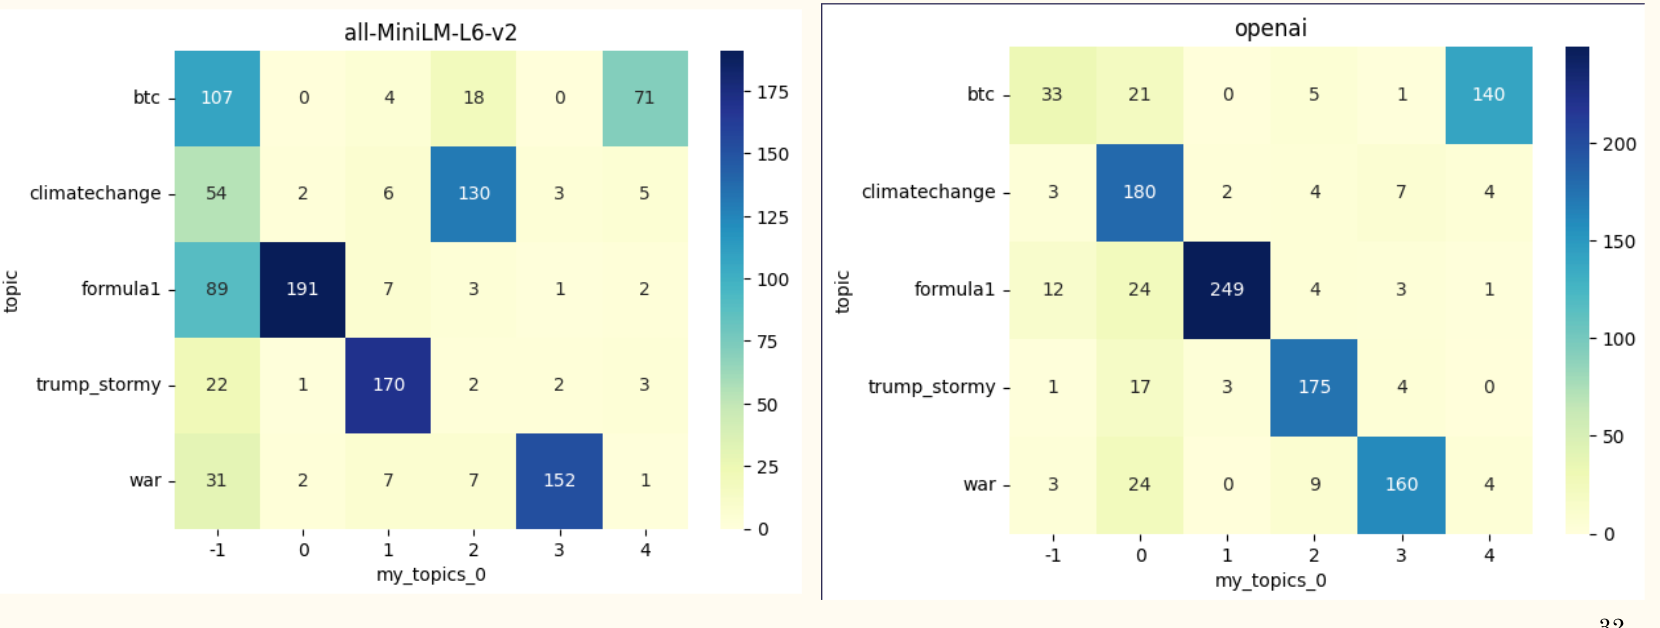
\includegraphics[width=0.99\linewidth]{Chapter4/figures/topic_heatmap_bertopic.png} 
    \caption{Heatmap comparison of mini and OpenAi of the simple dataset without hashtags}
    \label{figure:supervised heatmap1} % assign a unique label to each figure
\end{figure}
An interesting feature of Bertopic is the ability to visualize the different topics in a 2-dimensional space, Fig \ref{fig:openai docs} show the document distribution of OpenAi after projecting the embeddings in a two-dimensional space.
\begin{figure}
    \centering
    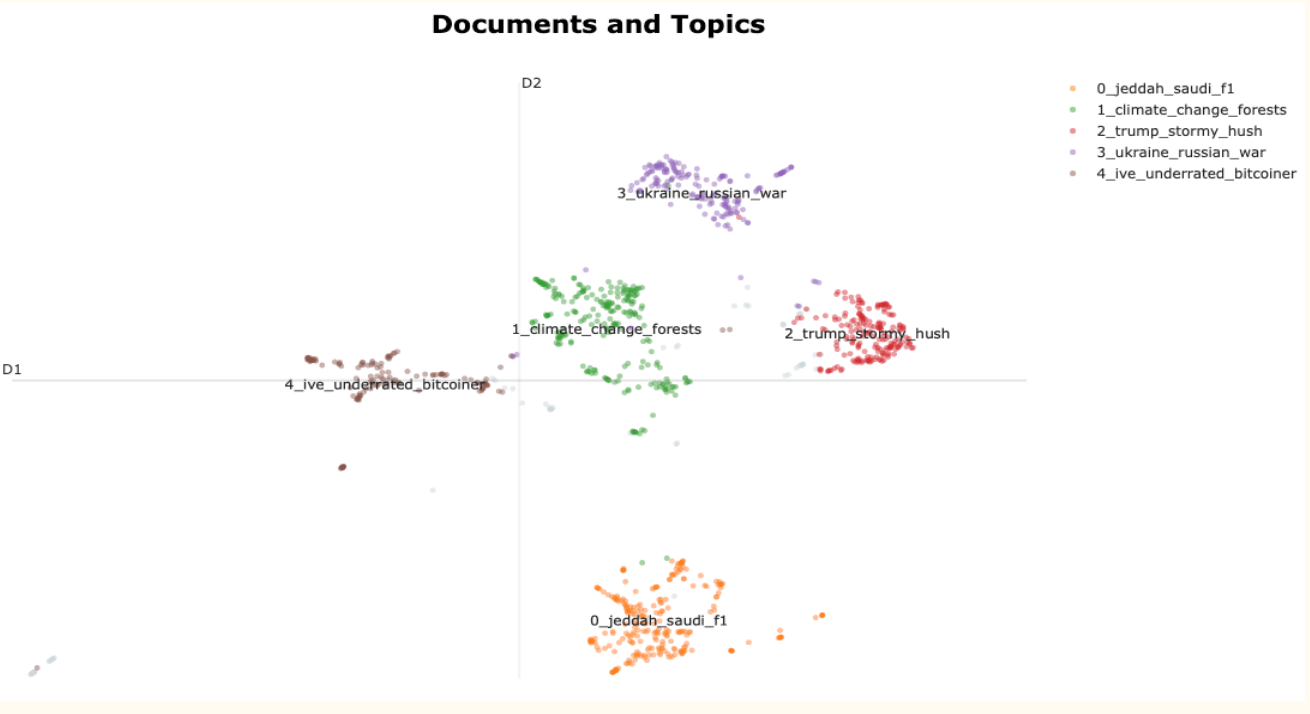
\includegraphics[width=1\linewidth]{Chapter4/figures/openai_documents_viz.png}
    \caption{docs representation of simple dataset for openai}
    \label{fig:openai docs}
\end{figure}


\paragraph{Politics dataset results}

The politics dataset is clearly more difficult to evaluate but with the hashtags it is still doing a good job. Even though we can see that both BERT and OpenAi are merging two topics. In particular, for OpenAi makes more sense since the two hashtags related to Trump are related to the same event( \#trump and \#trump\_stormy

\begin{figure}
    \centering
    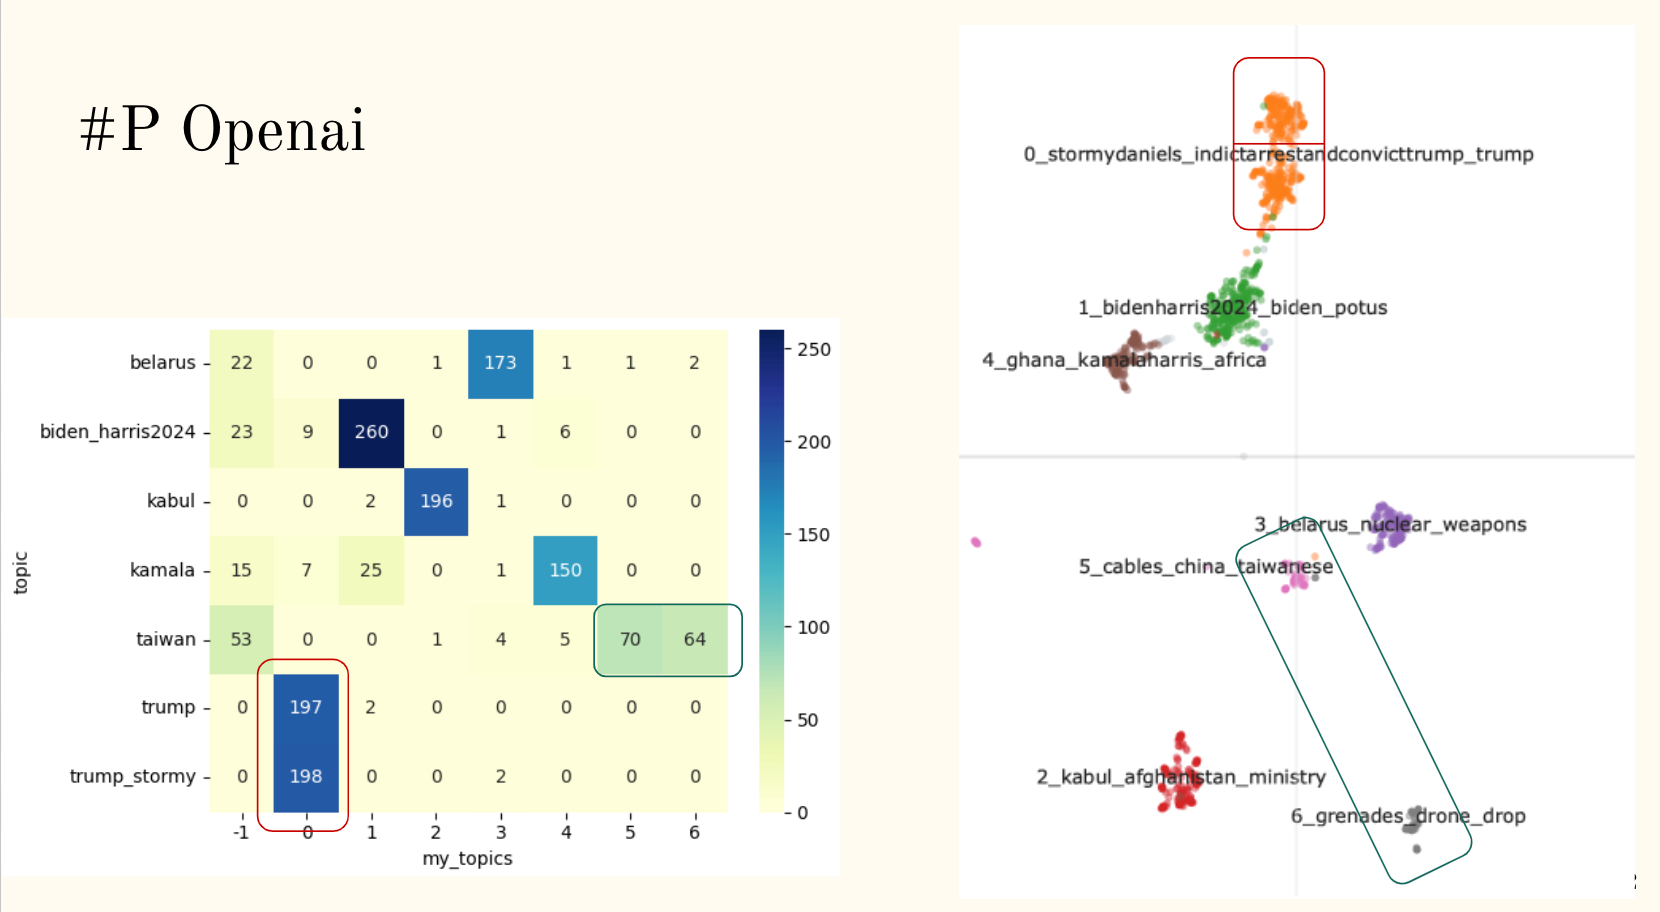
\includegraphics[width=1\linewidth]{Chapter4/figures/openai_politics_hash_comparison.png}
    \caption{Heatmap and documents representation of the politics dataset with hashtags evaluated with openai}
    \label{fig:openai_heat_docs_politics_hash}
\end{figure}

To validate the results we run the algorithm 100 times and most of the time for BERT the min topic share is 0.9 which means they got the correct number of topics and classified them in a good way. We can look at Fig \ref{fig:bert politics with hashtags} to see both documents and the heatmap.

\begin{figure}
    \centering
    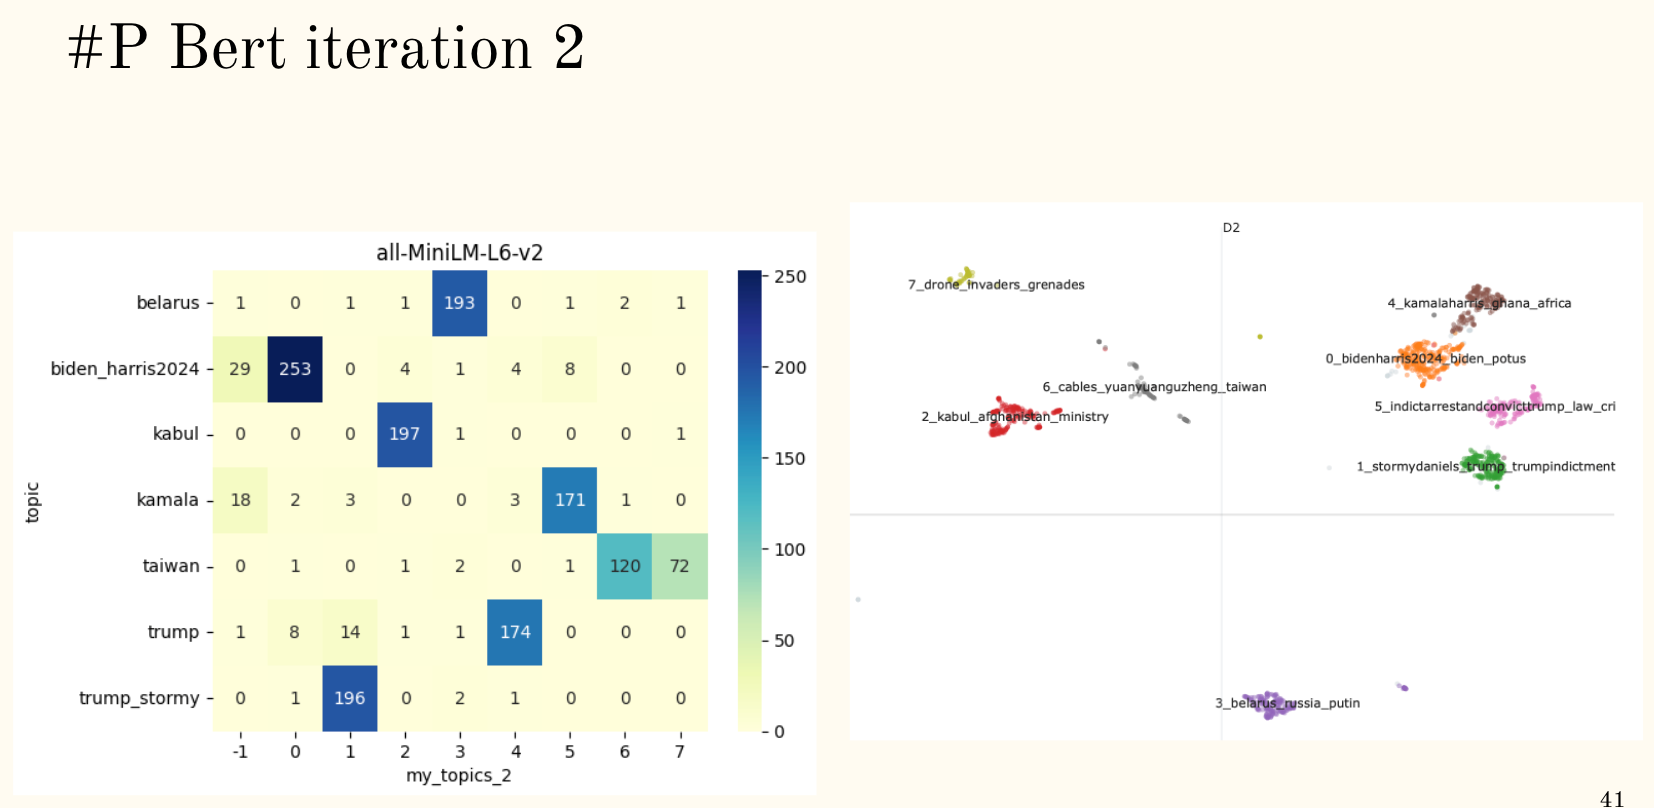
\includegraphics[width=1\linewidth]{Chapter4/figures/bert_politics_hash_comparison.png}
    \caption{bert heatmap and document viz politics with hashtags}
    \label{fig:bert politics with hashtags}
\end{figure}
in the case without hashtags OpenAi and BERT put in a single cluster all the tweets related to American politics both also understanding that Kamala's tweets were about something else.

\paragraph{Conclusion}
Tab \ref{tab:unsupervised_recap} show the result of unsupervised evaluation, while Tab \ref{tab:supervised recap } the supervised


\begin{table}[]
\centering
\begin{tabular}{|llll|}
\hline
\textbf{model}                              & \textbf{npmi} & \textbf{umass} & \textbf{diversity} \\ \hline
\multicolumn{1}{|l|}{tweet\_classification} & 0.62          & -0.16          & 1                  \\
\multicolumn{1}{|l|}{openai}                & 0.58          & -0.63          & 0.99               \\
\multicolumn{1}{|l|}{climatebert}           & 0.20          & -2.28          & 0.83               \\
\multicolumn{1}{|l|}{U.S.E}                 & 0.20          & -4.35          & 0.89               \\
\multicolumn{1}{|l|}{BERT}                  & 0.20          & -5.46          & 0.97               \\
\multicolumn{1}{|l|}{LDA}                   & -0.04         & -3.07          & 0.19               \\
\multicolumn{1}{|l|}{NMF}                   & -0.06         & -5.80          & 0.42               \\ \hline
\end{tabular}
\caption{all the models tested in the unsupervised evaluation}
\label{tab:unsupervised_recap}
\end{table}

\begin{table}[]
\centering
\begin{tabular}{|l|ll|}
\hline
model  & accuracy & topic share \\ \hline
BERT   & 0.84     & 0.86        \\
OpenAI & 0.83     & 0.85        \\
NMF    & 0.78     & 0.69        \\ \hline
\end{tabular}
\caption{recap of supervised evaluation}
\label{tab:supervised recap }
\end{table}


